\chapter{Serwis społecznościowy Twitter}
Serwis spo\l{}eczno\'sciowy Twitter jest globalnym serwisem internetowym s\l{}u\.z\k{a}cym g\l{}\'ownie do zamieszczania wiadomo\'sci tzw. \textit{tweet}, kt\'ore u\.zytkownicy tego serwisu mog\k{a} także czytać, komentowa\'c lub przekazywa\'c dalej. Od kilku lat Twitter jest serwisem gdzie dochodzi do wymiany zdań na różny temat, dotyczących np. polityki, sportu, produktów, wydarzeń społecznych, a profile posiada wiele osób znanych publicznie oraz instytucji.

\section{Historia}
Serwis ten, nazywany SMS internetu, zosta\l{} za\l{}o\.zony w 2006 r. w Stanach Zjednoczonych przez Jacka Dorseya, Ev Williamsa, Noah Glassa oraz Biza Stone’a i od początku powstania sukcesywnie zwi\k{e}ksza\l{} swoj\k{a} popularno\'s\'c poprzez wzrost liczby u\.zytkownik\'ow odwiedzaj\k{a}cych jego witryn\k{e} oraz wysy\l{}aj\k{a}cych wiadomo\'sci. W 2012 r. osiągnął ponad 100 milionów użytkowników, którzy zamieszczali łącznie ponad 340 milionów wiadomo\'sci dziennie oraz obsługiwał \'srednio około 1.6 miliarda wyszukujących zapytań dziennie. W 2013 r. Twitter stał si\k{e} jedną z najcze\'sciej odwiedzanych stron w całym internecie. W tym samym roku inżynierowie Twittera podali informację, że serwis ten obsługuje ok. 143 tys. wiadomości na sekundę. Na początku 2016 r. serwis ten posiadał ponad 319 milionów użytkowników aktywnych podczas każdego miesiąca. Od listopada 2013 r. akcje Twittera są obecne na nowojorskiej giełdzie.

\section{Tweet}
Tweet, czyli krótka wiadomość tekstowa, by\l{}a pocz\k{a}tkowo ograniczona do 140 znak\'ow, ale limit ten zosta\l{} podwojony w 2017 r. dla wszystkich j\k{e}zyk\'ow opr\'ocz chi\'nskiego, japo\'nskiego i korea\'nskiego. Użytkownicy mają możliwość wyróżniania wybranych przez siebie tematów przez dodanie do nich znaku '\#', co czyni takie wyrażenie tagiem. Inną możliwością oferowaną przez Twittera jest odpowiadanie innym użytkownikom lub zamieszczenie referencji do nich przez dodanie znaku '@' poprzedzającego nazwę profilu innej osoby.

\section{Architektura}
Serwis społecznościowy Twitter opierał się początkowo o typową architekturę trójwarstwową składająca się z warstwy prezentacji, logiki biznesowej oraz warstwy danych. Do napisania tej aplikacji został użyty framework Ruby on Rails wykorzystujący język Ruby, a warstwa bazodanowa opierała się o technologię MySQL. Jednak wraz ze wzrostem ilości przetwarzanych danych inżynierowie Twittera podjęli decyzję w 2011 r. o zmianie technologii na język Scala, który działa na maszynie wirtualnej Javy oraz zrezygnowano z dotychczasowej architektury na rzecz budowy rozproszonych serwisów komunikujących się między sobą. Wraz z przeprowadzonymi zmianami zanotowano ponad 10-krotne polepszenie obsługi tweetów.

\section{API}
Twitter jest platformą otwartą i udostępnia programowalny interfejs API w dwóch postaciach: Search API oraz Streaming API.

\subsection{Zakres działania}
Programiści korzystający z Search API są w stanie uzyskać dostęp tylko do danych historycznych, które zostały już wcześniej zamieszczone na łamach serwisu Twitter. Natomiast w przypadku Streaming API dostajemy możliwość śledzenia strumienia danych, które są do naszego dostępu nawet już kilka sekund po zamieszczeniu w serwisie Twitter. Po podłączeniu do takiego strumienia możemy cały czas obserwować nowe wiadomości. Przyjęło się stosować nazywnictwo, że analiza Search API to analiza \textit{back in time}, a Streaming API to śledzenie \textit{real time}.

\subsection{Rejestracja}
Obie formy API wymagają wcześniejszej rejestracji na stronie \textit{https://developer.twitter.com/en/apply-for-access} przeznaczonej dla deweloperów zainteresowanych wykorzystywaniem Twitter API. Po przejściu pomyślnej rejestracji dostajemy dane, które po nawiązaniu połączenia z serwisem Twitter umożliwiają mu jednoznacznie określić, że możemy uzyskać dostęp do API.

\subsection{Sposób działania}
Search API powstało z wykorzystaniem standardu REST - \textit{Representational State Transfer}. Oba rodzaje API wykorzystują protokół HTTP: do poprawnego działania Streaming API potrzebne jest ciągłe połączenie HTTP, a w przypadku drugiego z nich każda operacja jest wykonywana przy nawiązaniu oddzielnego połaczenia.

\begin{figure}[h] % h means here
	\centering
	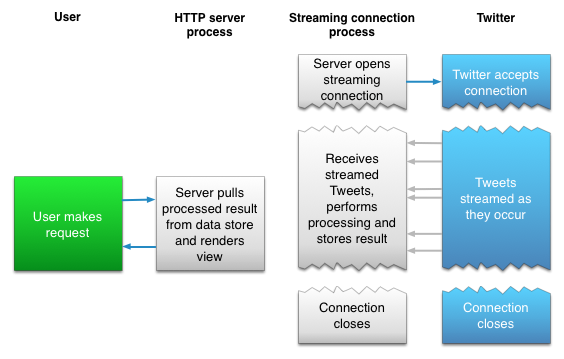
\includegraphics[width=0.6\linewidth]{img/twitter_api_comparison}
	\caption{Schemat działania dwóch rodzajów programistycznego interfejsu API udostępnianego przez serwis społecznościowy Twitter: Search API i Streaming API.}
\end{figure}

Search API posiada ściśle określone paramtery, które mogą być przesłane w żądaniu. W tabeli 3.1 zaprezentowano ich wykaz.

\begin{table}
\centering
\caption{Parametry żądania \textit{Twitter Search API} [3].}
\label{tab:table1}
\begin{tabularx}{\linewidth}{|c|c|X|c|}\toprule
    Parametr & {Wymagany/Opcjonalny} & {Opis} & {Przykład} \\ \midrule
    q & wymagany & {zapytanie wyszukujące o maksymalnej długości 500 znaków} & nasa \\ \midrule
    geocode & opcjonalny & {zwraca wiadomości użytkowników oddalonych o podany promień od podanej szerokości i długości geograficznej, promień może być podany w milach lub kilometrach} & {37.781157 -122.398720 1mi} \\ \midrule
    lang & opcjonalny & {ogranicza wiadomości do wybranego języka spośród dostępnych kodów ISO 639-1} & {pl} \\ \midrule
    locale & opcjonalny & {specyfikuje język wysyłanego zapytania, obecnie tylko \textit ja jest skuteczny} & {ja} \\ \midrule
    result\textunderscore type & opcjonalny & {określa typ zwracanych wiadomości, obecnie dostępne są trzy wartości tego parametru: \textit{recent} (zwracane są najnowsze wiadomości), \textit{popular} (zwracane są najbardziej popularne wiadomości) \textit{mixed} (wartość domyślna, zwracane wyniki obejmują najnowsze i najbardziej popularne wiadomości)} & {mixed} \\ \midrule
    count & opcjonalny & {specyfikuje ilość zwracanych wiadomości; maksymalna wartość to 100, a domyślna to 15} & 100 \\ \midrule
\end{tabularx}
\end{table}

\begin{table}
\centering
\label{tab:table1}
\begin{tabularx}{\linewidth}{|c|c|X|c|}\toprule
    until & opcjonalny & {ten parametr odpowiada za zwracanie wiadomości, których data utworzenia jest starsza o maksymalnie tydzień niż podana; obowiązuje format YYYY-MM-DD} & 2015-07-19  \\ \midrule
    since\textunderscore id & opcjonalny & {dzięki temu parametrowi zwracane są wiadomości o ID większym niż podane czyli nowsze wiadomości niż określono} & 12345   \\ \midrule
    max\textunderscore id & opcjonalny & {dzięki temu parametrowi zwracane są wiadomości o ID mnijeszym lub równym niż podane czyli starsze lub takie same wiadomości niż określono} & 54321 \\ \bottomrule
\end{tabularx}
\end{table}


Streaming API nie posiada takich ograniczeń. W języku programowania Java dostępny jest pakiet \textit{twitter4j} zawierający interfejsy \textit{User} oraz \textit{Status}, na które mapowane są przychodzące ze strumienia informacje. W tabeli 3.2 zamieszczam ich dokumentację.

\begin{table}
\centering
\caption{Dokumentacja interfejsu Status}
\label{tab:table1}
\begin{tabularx}{\linewidth}{|c|c|X|}\toprule
    Typ zwracany & Nazwa metody & Opis \\ \midrule
    long[] & getContributors() & \\ \midrule
    java.util.Date & getCreatedAt() & zwraca datę utworzenia wiadomości \\ \midrule 
    long & getCurrentUserRetweetId() & zwraca id użytkownika, którego wiadomość została podana dalej \\ \midrule
    int & getDisplayTextRangeEnd() & \\ \midrule 
    int & getDisplayTextRangeStart() & \\ \midrule
    int & getFavoriteCount() & zwraca informację ile razy została polubiona wiadomość \\ \midrule
    GeoLocation & getGeoLocation() & zwraca lokalizację użytkownika zamieszczającego tą wiadomość \\ \midrule 
    long & getId() & zwraca id wiadomości \\ \midrule
    java.lang.String & getInReplyToScreenName() & zwraca nazwę użytkownika, do którego kierowana jest odpowiedź \\ \midrule
    long & getInReplyToStatusId() & zwraca id wiadomości, do którego kierowana jest odpowiedź \\ \midrule 
    java.lang.String & getLang() & zwraca język zamieszczonej wiadomości \\ \midrule
    Place & getPlace() & zwraca obiekt Place przypisany do tej wiadomości \\ \midrule 
    Status & getQuotedStatus() & zwraca obiekt Status cytowanej wiadomości \\ \midrule
    long & getQuotedStatusId() & zwraca id cytowanej wiadomości \\ \midrule
    URLEntity & getQuotedStatusPermalink() & zwraca obiekt URLEntity reprezentujący bezpośredni odnośnik do cytowanej wiadomości \\ \midrule
    int & getRetweetCount() & zwraca ile razy wiadomość została podana dalej \\ \midrule
    Status & getRetweetedStatus()  & zwraca oryginalny status, który jest podany dalej w tej wiadomości \\ \midrule
    Scopes & getScopes() & zwraca obiekt typu Scopes posiadający informację o id miejsc, do których odnosi się ta wiadomość \\ \midrule
    java.lang.String & getSource() & zwraca źródło wiadomości \\ \midrule
    java.lang.String & getText() & zwraca tekst wiadomości \\ \midrule
    User & getUser() & zwraca obiekt typu User powiązany z tą wiadomością \\ \midrule
    java.lang.String[] & getWithheldInCountries() & zwraca tablicę nazw krajów, w których wiadomość została wstrzymana \\ \midrule
\end{tabularx}
\end{table}

\begin{table}
\centering
\label{tab:table1}
\begin{tabularx}{\linewidth}{|c|c|X|c|}\toprule 
    boolean & isFavorited() & zwraca informację czy wiadomość została polubiona \\ \midrule
    boolean & isPossiblySensitive() & zwraca informację czy wiadomość zawiera link do chronionych informacji \\ \midrule
    boolean & isRetweet() & zwraca informację czy tweet jest podaną dalej wiadomością \\ \midrule
    boolean & isRetweeted() & informuje czy wiadomość jest podana dalej \\ \midrule
    boolean & isRetweetedByMe() & informuje czy wiadomość jest podana dalej przez tego użytkownika \\ \midrule
    booleand & isTruncated() & informuje czy wiadomość jest skrócona (zakończona znakiem "...") \\ \bottomrule
\end{tabularx}
\end{table}

\begin{table}
\centering
\caption{Dokumentacja interfejsu User z pakietu twitter4j [6]. Zamieszczone zostały tylko najważniejsze z metod.}
\label{tab:table1}
\begin{tabularx}{\linewidth}{|c|c|X|}\toprule
    Typ zwracany & Nazwa metody & Opis \\ \midrule
    java.util.Date & getCreatedAt() & zwraca datę utworzenia profilu użytkownika \\ \midrule
    java.lang.String & getDescription() & zwraca opis konta użytkownika \\ \midrule
    java.lang.String & getEmail() & zwraca adres e-mail powiązany z tym kontem \\ \midrule
    int & getFavouritesCount() & zwraca liczbę wiadomości, którą polubił ten użytkownik \\ \midrule
    int & getFollowersCount() & podaje ilość użytkowników śledzących profil \\ \midrule
    int & getFriendsCount() & podaje ilość śledzonych profili \\ \midrule
    long & getId() & zwraca id użytkownika \\ \midrule
    java.lang.String & getLang() & zwraca język preferowany przez użytkownika \\ \midrule
    java.lang.String & getLocation() & zwraca lokalizację użytkownika \\ \midrule
    java.lang.String & getName() & podaje nazwę użytkownika \\ \midrule
    java.lang.String & getScreenName() & zwraca nazwę konta \\ \midrule
    Status & getStatus() & zwraca obiekt typu Status reprezentujący wiadomość wysłaną przez użytkownika \\ \midrule
    int & getStatusesCount() & podaje ilość wiadomości wysłanych przez użytkownika \\ \midrule
    java.lang.String & getTimeZone() & podaje strefę czasową użytkownika \\ \midrule
    java.lang.String & getURL() & zwraca URL do profilu \\ \midrule
    boolean & isVerified() & podaje informację czy profil jest zweryfikowany \\ \bottomrule 
\end{tabularx}
\end{table}


\subsection{Ograniczenia}
Korzystając z Search API mamy możliwość wysłania 720 zapytań na godzinę, a maksymalna ilość wiadomości jaka może być zwrócona na jedno zapytanie to 100. Jeśli wykorzystalibyśmy ten limit w maksymalny sposób to daje nam to 72 000 wiadomości na godzinę. W przypadku Streaming API głównym ograniczeniem jest dostęp do ok. 1 \% danych ze strumienia, a maksymalna ilość wiadomości w czasie jednej minuty to 3 000. W przypadku tego API w ciągu godziny możemy uzyskać 180 000 wiadomości na godzinę. Są to ograniczenia, które obowiązują dla rozwiązań typu \textit{open-source}.

\section{Dostępne narzędzia analityczne}
Udostępnienie API przez serwis społecznościowy Twitter oraz rosnące znaczenie danych generowanych przez użytkowników tego serwisu spowodowało, że wiele firm oraz instytucji zaczęło przywiązywać dużą wagę do analizy opinii wyrażanych na swój temat lub na tematy pokrewne, zainteresowania pewnymi tematami oraz kształtujących się trendów. Dlatego powstały aplikacje internetowe służące do wyświetlania takich informacji i przeprowadzające wstępną analizę zebranych danych. W dalszej części pracy znajduje się omówienie najważniejszych z nich.

\subsection{Twitter Analytics}

Pierwszym z narzędzi, którym warto poświęcić uwagę jest \textit{Twitter Analytics}. Aplikacja ta posiada trzy zakładki. Na pierwszej z nich wyświetla statystyki dotyczące profilu z serwisu Twitter, którym logujemy się do niej: naszą najbardziej popularną wiadomość, najpopularniejszą wzmiankę o naszym profilu oraz wykresy trendów m. in. liczby osób śledzących nasz profil i odwiedzin. Na kolejnej zakładce mamy możliwość tworzenia wiadomości, które zostaną wygenerowane na naszym profilu oraz dodania do nich plików graficznych, materiałów audio lub wideo. Na ostatniej stronie użytkownik ma szansę poznania informacji takich jak np. lokalizacja geograficzna i wiek osób śledzących nasz profil czyli tzw. \textit{followers}.

\begin{figure}[h] % h means here
	\centering
	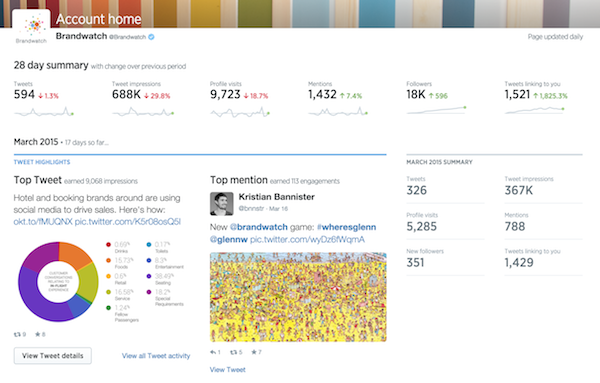
\includegraphics[width=0.8\linewidth]{img/twitter_tool_twitter_analytics}
	\caption{Narzędzie Twitter Analytics.}
\end{figure}

\subsection{Hootsuite}

Kolejną aplikacją jest \textit{Hootsuite}. Jest to narzędzie, które umożliwia prowadzić kampanie w kilku mediach społecznościowych na raz np. \textit{Facebook}, \textit{Instagram}, \textit{Linkedin}. Posiada wiele rozbudowanych funkcji. Co ciekawe Hootsuite pozwala na analizę nastrojów społecznych dla wybranych słów kluczowych. Wyświetlane informacje zawierają ogólny zarys użytkowników zamieszczających wiadomości na dany temat np. lokalizację geograficzną, podział ze względu na płeć i język oraz wykres trendu. Aplikacja ta wyświetla wszystkie wiadomości, w których użytkownicy używają wybranego słowa kluczowego. Jak podają twórcy tego narzędzia ma to główne zastosowanie jako pomoc w kampaniach marketingowych w dotarciu do użytkowników krytykujących produkt i posiadających największą ilością osób śledzących.

\begin{figure}[h] % h means here
	\centering
	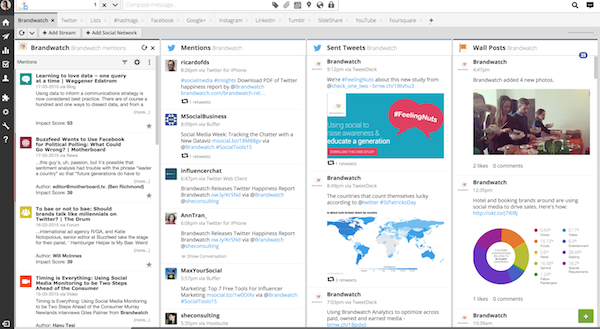
\includegraphics[width=0.8\linewidth]{img/twitter_tool_hootsuite}
	\caption{Narzędzie Hootsuite - główny pulpit.}
\end{figure}

\begin{figure}[h] % h means here
	\centering
	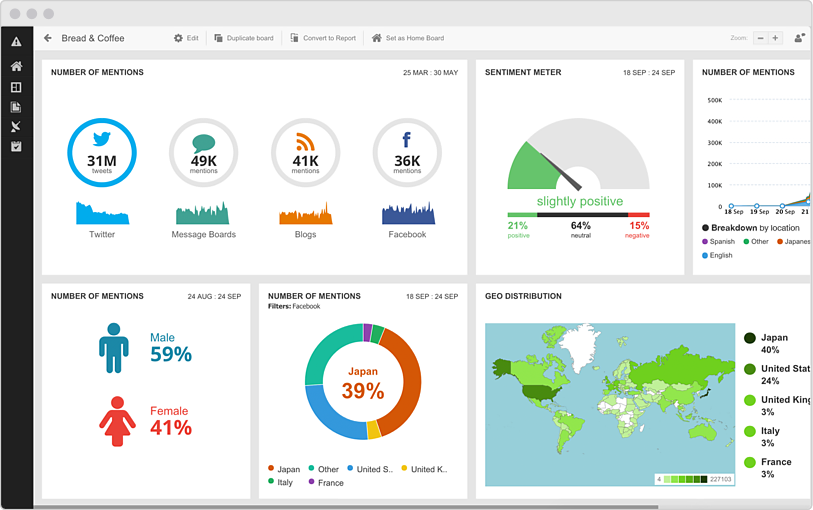
\includegraphics[width=0.8\linewidth]{img/twitter_tool_hootsuite_insights}
	\caption{Narzędzie Hootsuite - badanie nastrojów społecznych.}
\end{figure}

\subsection{Mentionmap}

Trzecim narzędziem wartym omówienia jest \textit{Mentionmap}. Jest to aplikacja, która wyróżnia się spośród innych tym, że rysuje wykres powiązań pomiędzy użytkownikami wchodzącymi w interakcje z danym profilem, a także z ich profilami. Posiada także podstronę umożliwiającą badanie nastrojów społecznych osób zamieszczających wiadomości z konkretnym słowem kluczowym. Nastroje te są przedstawione w postaci chmury nazw kont użytkowników, gdzie kolor nazwy zależy od nastoroju prezentowanego przez użytkownika pod kątem słowa kluczowego.

\begin{figure}[h] % h means here
	\centering
	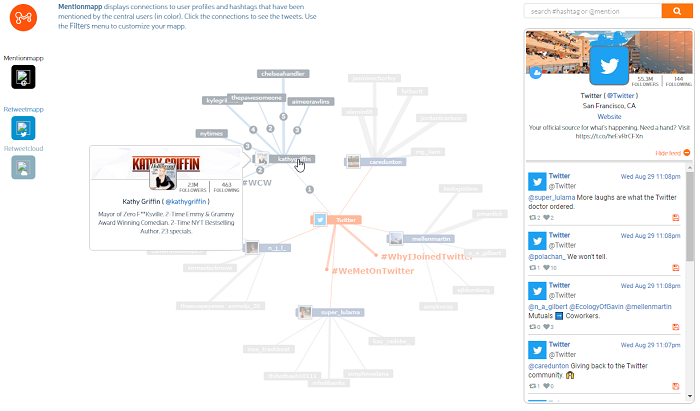
\includegraphics[width=0.8\linewidth]{img/twitter_tool_mentionmap}
	\caption{Narzędzie Mentionmap - wykres powiązań.}
\end{figure}

\begin{figure}[h] % h means here
	\centering
	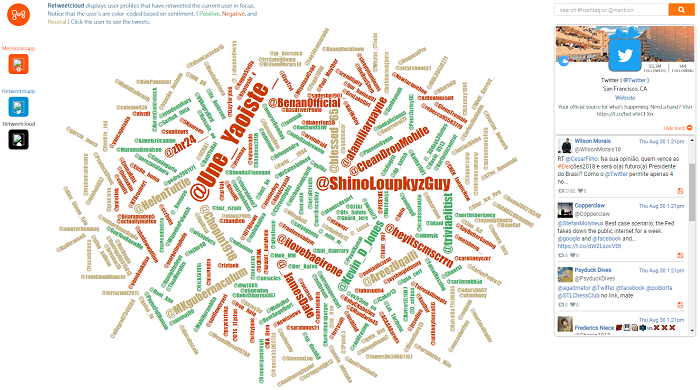
\includegraphics[width=0.8\linewidth]{img/twitter_tool_mentionmap_sentiment}
	\caption{Narzędzie Mentionmap - badanie nastrojów społecznych.}
\end{figure}

\subsection{Podsumowanie}

Podsumowując warto zauważyć, że nie ma obecnie na rynku aplikacji, która umożliwiałaby śledzenie występowania dowolnego słowa w wiadomościach zamieszczanych w czasie rzeczywistym w serwisie Twitter, rysowałaby wykres zależności pomiędzy użytkownikami tego serwisu, analizowałaby nastroje społeczne użytkowników z wyświetleniem informacji o nastroju wyrażanym w poszczególnych wiadomościach oraz pozwalałaby na analizowanie danych historycznych i zamieszczanych w czasie rzeczywistym. Taka sytuacja pozwala na utworzenie nowej aplikacji, która udostępniałaby te funkcjonalności. 